\documentclass[12pt,a4paper]{article}

\usepackage[utf8]{inputenc}
\usepackage[T1]{fontenc}
\usepackage{geometry}
\usepackage{amsmath,amssymb,amsthm}
\usepackage{array,booktabs,longtable,multirow}
\usepackage{enumitem}
\usepackage{tikz}
\usetikzlibrary{automata,positioning,arrows.meta}
\usepackage{mathtools}
\usepackage{fancyhdr}
\usepackage{lastpage}

\geometry{margin=1in}
\setlength{\parskip}{0.5em}
\setlength{\parindent}{0pt}

\pagestyle{fancy}
\fancyhf{}
\fancyhead[L]{Computer Hardware --- Final Examination Solution}
\fancyhead[R]{Semester II, 2022--2023}
\fancyfoot[C]{\thepage/\pageref{LastPage}}

\begin{document}

\begin{center}
    {\LARGE \textbf{Test-Style Solution}}\\[0.5em]
    {\large VNUHCM--University of Science}\\
    {\large Course: Computer Hardware (ECE341)}
\end{center}

\hrule
\vspace{1em}

\textbf{Remark for Question 3:} the statement on Page 3 appears slightly inconsistent with the data on Page 2.  
To keep the solution coherent, the standard interpretation is used:
\[
\texttt{Load R4, 200(R3)} \Rightarrow R4 \leftarrow M[R3+200].
\]
With \(R3=28000\), this means address \(28200\), hence \(R4 \leftarrow 500\).

\section*{Question 1 (25 points)}

Three processors execute the same ISA:

\[
\begin{aligned}
P1 &: f_1 = 3~\text{GHz},\quad \text{CPI}_1 = 2.5,\\
P2 &: f_2 = 2.5~\text{GHz},\quad \text{CPI}_2 = 1.0,\\
P3 &: f_3 = 4.0~\text{GHz},\quad \text{CPI}_3 = 2.2.
\end{aligned}
\]

Recall:
\[
\text{IPS} = \frac{\text{Clock rate}}{\text{CPI}}.
\]

\subsection*{(a) Highest performance in instructions/second}

\[
\text{IPS}_1=\frac{3\times 10^9}{2.5}=1.2\times 10^9
\]
\[
\text{IPS}_2=\frac{2.5\times 10^9}{1.0}=2.5\times 10^9
\]
\[
\text{IPS}_3=\frac{4\times 10^9}{2.2}\approx 1.818\times 10^9
\]

Therefore,
\[
\boxed{P2 \text{ has the highest performance}}
\]
with
\[
\boxed{2.5\times 10^9\ \text{instructions/s}}.
\]

\subsection*{(b) If each processor executes for 15 seconds, find cycles and instructions}

Use
\[
\text{Cycles} = f \cdot T,\qquad
\text{Instructions} = \frac{\text{Cycles}}{\text{CPI}}.
\]

\paragraph{Processor \(P1\):}
\[
\text{Cycles}_1 = 3\times 10^9 \times 15 = 45\times 10^9
\]
\[
\text{Instructions}_1=\frac{45\times 10^9}{2.5}=18\times 10^9
\]

\paragraph{Processor \(P2\):}
\[
\text{Cycles}_2 = 2.5\times 10^9 \times 15 = 37.5\times 10^9
\]
\[
\text{Instructions}_2=\frac{37.5\times 10^9}{1.0}=37.5\times 10^9
\]

\paragraph{Processor \(P3\):}
\[
\text{Cycles}_3 = 4\times 10^9 \times 15 = 60\times 10^9
\]
\[
\text{Instructions}_3=\frac{60\times 10^9}{2.2}\approx 27.273\times 10^9
\]

Hence:
\[
\boxed{
\begin{array}{c|c|c}
\text{Processor} & \text{Cycles} & \text{Instructions} \\
\hline
P1 & 45\times 10^9 & 18\times 10^9 \\
P2 & 37.5\times 10^9 & 37.5\times 10^9 \\
P3 & 60\times 10^9 & 27.273\times 10^9
\end{array}}
\]

\subsection*{(c) Reduce execution time by 40\% while CPI increases by 30\%}

Original time:
\[
T=\frac{IC\cdot CPI}{f}
\]

New constraints:
\[
T' = 0.6T,\qquad CPI' = 1.3\,CPI
\]

Then
\[
T'=\frac{IC\cdot CPI'}{f'}=\frac{IC\cdot 1.3\,CPI}{f'}
\]
and also
\[
T' = 0.6\frac{IC\cdot CPI}{f}
\]

Equating:
\[
\frac{1.3}{f'}=\frac{0.6}{f}
\quad\Rightarrow\quad
f'=\frac{1.3}{0.6}f=\frac{13}{6}f\approx 2.1667f
\]

So each processor would require:

\[
f_1' = 2.1667 \times 3 = 6.5~\text{GHz}
\]
\[
f_2' = 2.1667 \times 2.5 \approx 5.417~\text{GHz}
\]
\[
f_3' = 2.1667 \times 4 \approx 8.667~\text{GHz}
\]

Therefore,
\[
\boxed{f' = 2.1667f}
\]
and specifically:
\[
\boxed{
P1: 6.5~\text{GHz},\quad
P2: 5.417~\text{GHz},\quad
P3: 8.667~\text{GHz}
}
\]

\newpage
\section*{Question 2 (25 points)}

\subsection*{Question 2-1}

A 5-stage pipelined RISC processor \(C1\) runs at \(2.6\text{ GHz}\).

Instruction mix:
\[
\text{Branches}=10\%,\quad
\text{Loads}=20\%,\quad
\text{Stores}=20\%,\quad
\text{Arithmetic}=50\%
\]

Other information:
\begin{itemize}[leftmargin=2em]
    \item No data dependencies.
    \item Branch predictor accuracy \(=85\%\).
    \item Branch outcome resolved in stage 3.
    \item 100\% instruction fetches hit cache.
    \item 100\% data writes hit cache.
    \item 98\% data reads hit cache.
    \item Total instruction count \(=20\) billion.
    \item Required execution time \(<10\) seconds.
\end{itemize}

Let the main-memory miss penalty be \(P\) cycles.

\subsubsection*{Step 1: Ideal CPI}

For a perfect 5-stage pipeline without stalls,
\[
CPI_{\text{ideal}} = 1.
\]

\subsubsection*{Step 2: Branch penalty contribution}

Misprediction rate:
\[
1-0.85=0.15
\]

Branches are \(10\%\) of instructions, so mispredicted branches are:
\[
0.10\times 0.15=0.015
\]

Since the actual outcome is known in stage 3, a wrong prediction flushes the instructions in stages 1 and 2.  
Thus, the penalty is taken as \(2\) cycles per misprediction.

So branch CPI overhead is:
\[
\Delta CPI_{\text{branch}} = 0.015\times 2 = 0.03
\]

\subsubsection*{Step 3: Load-miss penalty contribution}

Loads are \(20\%\) of all instructions.

Load miss rate:
\[
1-0.98=0.02
\]

Thus the fraction of instructions causing a load miss is:
\[
0.20\times 0.02=0.004
\]

Each miss costs \(P\) cycles, hence:
\[
\Delta CPI_{\text{mem}} = 0.004P
\]

\subsubsection*{Step 4: Total CPI}

\[
CPI = 1 + 0.03 + 0.004P = 1.03 + 0.004P
\]

\subsubsection*{Step 5: Time constraint}

Execution time:
\[
T=\frac{IC\cdot CPI}{f}
\]

Substitute:
\[
10 \ge \frac{20\times 10^9 \cdot CPI}{2.6\times 10^9}
\]

So
\[
CPI \le \frac{10\cdot 2.6\times 10^9}{20\times 10^9}=1.3
\]

Thus:
\[
1.03 + 0.004P \le 1.3
\]
\[
0.004P \le 0.27
\]
\[
P \le \frac{0.27}{0.004}=67.5
\]

Hence the upper bound is
\[
\boxed{P_{\max}=67.5\ \text{cycles}}
\]

If an integer number of cycles is required:
\[
\boxed{P_{\max}=67\ \text{cycles}}
\]

\subsection*{Question 2-2}

Design a Mealy FSM that detects serial input patterns:
\begin{itemize}[leftmargin=2em]
    \item output \(z=10\) when data \(=1101\),
    \item output \(z=01\) when data \(=1110\),
    \item otherwise \(z=00\),
\end{itemize}
including overlap.

\subsubsection*{State definition}

Use states corresponding to the longest suffix that is also a prefix of one of the target patterns.

\[
\begin{array}{c|l}
\text{State} & \text{Meaning} \\
\hline
S_0 & \epsilon \text{ (no useful prefix matched)}\\
S_1 & 1\\
S_{11} & 11\\
S_{110} & 110\\
S_{111} & 111
\end{array}
\]

\subsubsection*{State transition/output table}

\[
\boxed{
\begin{array}{c|c|c}
\text{Present state} & x=0 & x=1 \\
\hline
S_0   & S_0/00   & S_1/00 \\
S_1   & S_0/00   & S_{11}/00 \\
S_{11}& S_{110}/00 & S_{111}/00 \\
S_{110} & S_0/00 & S_1/10 \\
S_{111} & S_{110}/01 & S_{111}/00
\end{array}}
\]

\subsubsection*{Explanation of overlap handling}

\begin{itemize}[leftmargin=2em]
    \item From \(S_{110}\), if the next bit is \(1\), we detect \(1101\), so output is \(10\).  
    The ending suffix is \(1\), so the next state is \(S_1\).
    \item From \(S_{111}\), if the next bit is \(0\), we detect \(1110\), so output is \(01\).  
    The ending suffix is \(110\), so the next state is \(S_{110}\).
\end{itemize}

\subsubsection*{Optional state diagram (TikZ)}

\begin{center}
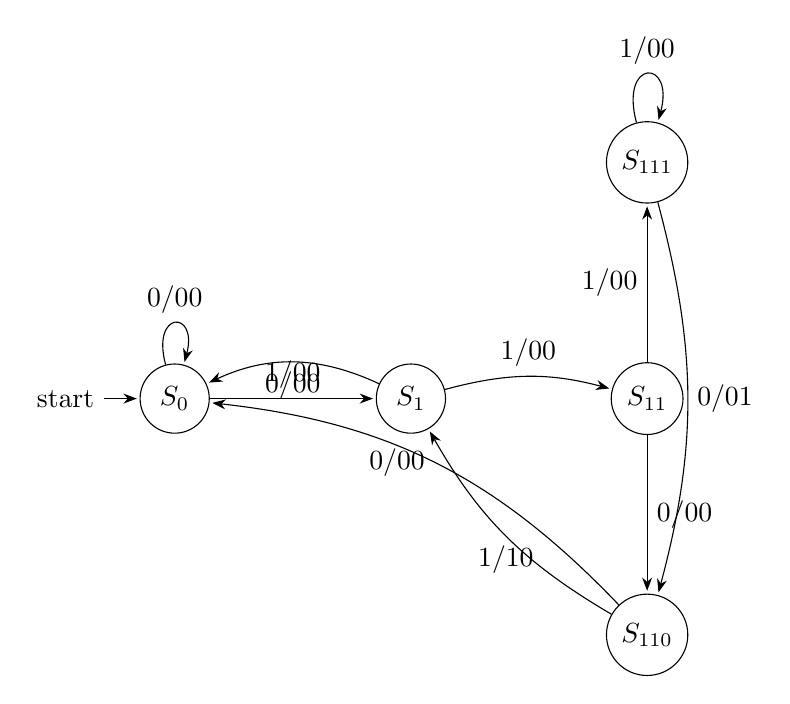
\begin{tikzpicture}[->,>=Stealth,shorten >=1pt,node distance=3cm,on grid,auto]
\node[state,initial] (S0) {$S_0$};
\node[state] (S1) [right=of S0] {$S_1$};
\node[state] (S11) [right=of S1] {$S_{11}$};
\node[state] (S110) [below=of S11] {$S_{110}$};
\node[state] (S111) [above=of S11] {$S_{111}$};

\path
(S0) edge[loop above] node {$0/00$} ()
     edge node {$1/00$} (S1)
(S1) edge[bend left=15] node {$1/00$} (S11)
     edge[bend right=25] node[below] {$0/00$} (S0)
(S11) edge node {$0/00$} (S110)
      edge node {$1/00$} (S111)
(S110) edge[bend right=20] node[left] {$0/00$} (S0)
       edge[bend left=15] node[below] {$1/10$} (S1)
(S111) edge[bend left=15] node[right] {$0/01$} (S110)
       edge[loop above] node {$1/00$} ();
\end{tikzpicture}
\end{center}

\newpage
\section*{Question 3 (25 points)}

Instruction sequence:
\[
\begin{aligned}
I_1 &: \texttt{Load R4, 200(R3)} \\
I_2 &: \texttt{Add R5, R2, R4} \\
I_3 &: \texttt{Store R5, 400(R3)}
\end{aligned}
\]

Given:
\[
R2=200,\quad R3=28000,\quad M[28000]=400,\quad M[28200]=500,\quad M[28400]=600
\]

Using the standard addressing interpretation:

\[
I_1:\quad R4 \leftarrow M[R3+200] = M[28200]=500
\]

Then:
\[
I_2:\quad R5 \leftarrow R2+R4 = 200+500=700
\]

Finally:
\[
I_3:\quad M[R3+400] \leftarrow R5 = M[28400]\leftarrow 700
\]

\subsection*{(a) For each instruction}

\subsubsection*{Instruction 1: \texttt{Load R4, 200(R3)}}

\begin{itemize}[leftmargin=2em]
    \item \textbf{MuxB selection:} immediate offset \(200\), so
    \[
    \boxed{\text{MuxB selects input 1 (immediate)}}
    \]
    \item \textbf{Stage 4 (\(RY\)):} load obtains memory data from \(M[28200]=500\), hence
    \[
    \boxed{RY=500}
    \]
    \item \textbf{Stage 5 (\(RF\_write\)):} load writes back into \(R4\), so
    \[
    \boxed{RF\_write=1}
    \]
\end{itemize}

\subsubsection*{Instruction 2: \texttt{Add R5, R2, R4}}

\begin{itemize}[leftmargin=2em]
    \item \textbf{MuxB selection:} second ALU operand comes from register \(R4\), so
    \[
    \boxed{\text{MuxB selects input 0 (register operand)}}
    \]
    \item \textbf{Stage 4 (\(RY\)):} ALU result is forwarded:
    \[
    RY = R2+R4 = 200+500=700
    \]
    therefore
    \[
    \boxed{RY=700}
    \]
    \item \textbf{Stage 5 (\(RF\_write\)):} add writes result into \(R5\), so
    \[
    \boxed{RF\_write=1}
    \]
\end{itemize}

\subsubsection*{Instruction 3: \texttt{Store R5, 400(R3)}}

\begin{itemize}[leftmargin=2em]
    \item \textbf{MuxB selection:} effective address uses immediate offset \(400\), so
    \[
    \boxed{\text{MuxB selects input 1 (immediate)}}
    \]
    \item \textbf{Stage 4 (\(RY\)):} the effective address is
    \[
    R3+400 = 28000+400=28400
    \]
    In the common 5-stage datapath convention, \(RY\) receives the pass-through ALU/address value in stage 4 for a store:
    \[
    \boxed{RY=28400}
    \]
    \item \textbf{Stage 5 (\(RF\_write\)):} store does not write a register, so
    \[
    \boxed{RF\_write=0}
    \]
\end{itemize}

\subsection*{(b) Final contents of memory locations 28400 and 28800}

Only the store updates memory:
\[
M[28400]\leftarrow 700
\]

No instruction accesses address \(28800\), so it remains unchanged.

Thus:
\[
\boxed{M[28400]=700}
\]
\[
\boxed{M[28800]\ \text{unchanged}}
\]

\newpage
\section*{Question 4 (25 points)}

Instruction sequence:
\[
\begin{aligned}
I_1 &: \texttt{LOAD R4, \#200(R2)} \\
I_2 &: \texttt{XOR R5, R3, R4} \\
I_3 &: \texttt{CALL\_REGISTER R5}
\end{aligned}
\]

Given:
\[
R2=2000,\quad R3=60,\quad R4=100,
\]
\[
M[2000]=10,\quad M[2200]=26
\]

\subsection*{Step 1: Execute instruction semantics}

\subsubsection*{Instruction 1: \texttt{LOAD R4, \#200(R2)}}

Effective address:
\[
R2+200 = 2000+200 = 2200
\]

So:
\[
R4 \leftarrow M[2200] = 26
\]

Thus the inter-stage ALU register after stage 3 is:
\[
\boxed{RZ_{(I_1)} = 2200}
\]

\subsubsection*{Instruction 2: \texttt{XOR R5, R3, R4}}

After \(I_1\), \(R4=26\). Hence:
\[
R5 \leftarrow R3 \oplus R4 = 60 \oplus 26
\]

In binary:
\[
60 = 00111100_2,\qquad 26 = 00011010_2
\]
\[
60\oplus 26 = 00100110_2 = 38
\]

So:
\[
\boxed{R5=38}
\]
and after stage 3:
\[
\boxed{RZ_{(I_2)} = 38}
\]

\subsubsection*{Instruction 3: \texttt{CALL\_REGISTER R5}}

The call target is the value in \(R5\), therefore the new PC becomes:
\[
\boxed{PC=38}
\]

\subsection*{Control signals}

From the datapath:
\begin{itemize}[leftmargin=2em]
    \item \(Y\_select\) chooses the value written into \(RY\):
    \begin{itemize}
        \item 0: ALU result / \(RZ\)
        \item 1: Memory data
        \item 2: Return address
    \end{itemize}
    \item \(RF\_write\) indicates whether a register is written in stage 5.
    \item \(C\_select\) chooses the destination register:
    \begin{itemize}
        \item 0: \(IR_{26\text{-}22}\)
        \item 1: \(IR_{21\text{-}17}\)
        \item 2: LINK
    \end{itemize}
\end{itemize}

\subsubsection*{Instruction 1: \texttt{LOAD R4, \#200(R2)}}

\begin{itemize}[leftmargin=2em]
    \item Load gets data from memory in stage 4:
    \[
    \boxed{Y\_select = 1}
    \]
    \item Load writes destination register in stage 5:
    \[
    \boxed{RF\_write = 1}
    \]
    \item For a load, the destination is the register field used as load destination:
    \[
    \boxed{C\_select = 0}
    \]
\end{itemize}

\subsubsection*{Instruction 2: \texttt{XOR R5, R3, R4}}

\begin{itemize}[leftmargin=2em]
    \item Arithmetic/logic instructions forward ALU result:
    \[
    \boxed{Y\_select = 0}
    \]
    \item XOR writes result into \(R5\):
    \[
    \boxed{RF\_write = 1}
    \]
    \item Destination register is the third field:
    \[
    \boxed{C\_select = 1}
    \]
\end{itemize}

\subsubsection*{Instruction 3: \texttt{CALL\_REGISTER R5}}

\begin{itemize}[leftmargin=2em]
    \item Call saves return address:
    \[
    \boxed{Y\_select = 2}
    \]
    \item Call writes the return address into LINK:
    \[
    \boxed{RF\_write = 1}
    \]
    \item Destination register is LINK:
    \[
    \boxed{C\_select = 2}
    \]
\end{itemize}

\subsection*{Final summary table}

\[
\boxed{
\begin{array}{c|c|c|c}
\text{Instruction} & Y\_select & RF\_write & C\_select \\
\hline
\texttt{LOAD R4,\#200(R2)} & 1 & 1 & 0 \\
\texttt{XOR R5,R3,R4} & 0 & 1 & 1 \\
\texttt{CALL\_REGISTER R5} & 2 & 1 & 2
\end{array}}
\]

Also,
\[
\boxed{RZ_{(I_1)} = 2200}
\]
\[
\boxed{RZ_{(I_2)} = 38}
\]
\[
\boxed{PC_{\text{final}} = 38}
\]

\vspace{1em}
\hrule
\vspace{0.5em}

\begin{center}
    \textbf{End of Solution}
\end{center}

\end{document}